% withtuning experiments
%     - freq exp
%     - iter exp
%     - analyze
% notuning exp
%     - vlc c08
%     - lc c08
%     - vcl c06
%     - why chosen? adv? how they work in tehcnical background
% percentage expr
%     - why only run in some of them
%     - why still not performat
%     - why chose to use spinodal all of a sudden 
%     - idea to converge to DVL
%     - is the slight improvement only a coincidence - repeating the tests many times
%     - idea to increase the temperatur in spinodial decomp 
% Profiler
% add where to find the tests on github and such, also attach slurm job maybe
%add in which cluster each experiment was ran on


This chapter explores whether the use of the fast particle buffer provides measurable advantages by presenting the results of various experiments conducted under different scenarios. It details the experimental setup, including the working environment, explains the rationale behind the selection of specific experiments, and provides an analysis of the observed outcomes. Due to the high number of experiments conducted, only the most relevant data and plots are presented here. However, the complete dataset, including the \texttt{.yaml} files and all scripts used for plotting, is available in the accompanying \href{https://github.com/xhulia028/GraphView}{\texttt{GitHub repository}}.

% ======================================================================
\section{Test System Specifications}

The initial experiments were conducted on the CoolMUC2 Linux cluster at the Leibniz Supercomputing Centre (LRZ), TUM. This cluster operated on the SLES15 SP1 Linux OS and consisted of 812 nodes, each equipped with 28 cores running at a nominal frequency of 2.6 GHz with two hyperthreads per core \parencite{coolmuc2}. The \texttt{cm2\_tiny} partition was used for these experiments. Unfortunately, due to a severe hardware failure, CoolMUC2 was decommissioned during the course of this work.

Subsequent experiments were performed on CoolMUC4, the successor to CoolMUC2. CoolMUC4 features Intel® Xeon® Platinum 8380 CPUs (Ice Lake) with 112 cores per node, 512 GB of RAM, and a nominal core frequency of 3.0 GHz (ranging from 0.8 to 4.2 GHz). It operates on the SLES15 SP6 Linux OS \parencite{coolmuc4}. The experiments were run on the \texttt{cm4\_tiny} partition.

The code was compiled with GCC 11.2.0 in CoolMuc2 and GCC 12.2.0 in CoolMuc4. 

\section{Deletion Function}

The additional delete function did not yield significant performance improvements. Its primary use case arises when tuning is enabled, yet for the majority of the experiments, as it will be explained throughout this section, tuning was turned off, making its impact minimal. Moreover, since the focus of this thesis is on Verlet Lists, which rely on neighbor lists, the function has limited applicability. In these types of containers, particles cannot be fully deleted but must instead be marked as dummy particles to maintain neighbor list integrity.  

The only scenario where this function could be beneficial is when tuning is enabled and a combination of Linked Cells and Verlet Lists is used, as it would primarily benefit Linked Cells. However, considering the primary focus of this work, the function was not extensively utilized. Additionally, implementing it introduced extra computational overhead and increased code complexity, as it required implementation across all container types in AutoPas, as described in the Implementation section.



% ======================================================================
\section{Scenario descriptions}

For the experiments, four different simulations were used, each chosen to assess the impact of the fast particle buffer under various conditions and provide a comprehensive evaluation of its performance.

% \textbf{TESTS CAN BE FOUND IN GITHUB}
% \textbf{Cite Luis' thesis for some of these details; the rest cite AutoPas.}


\subsection{Falling Drop} 
This experiment involves two objects: \texttt{CubeClosestPacked}, which represents a bed of particles, and a sphere of particles. At the start of the simulation, the sphere is accelerated by gravity and falls into the basin. Upon collision, the particles from the sphere mix with those in the basin. This experiment uses reflective boundaries and the Lennard-Jones AVX functor, containing over 15,000 particles. The default YAML configuration for this experiment is set to run for 15,000 iterations; however, as will be discussed later, this parameter is adjusted for specific tests. The initial and final states of the simulation are depicted below \ref{fig:fd}, illustrating the transition from the sphere's descent to the equilibrium state of the mixed particles.

\subsection{Exploding Liquid} The second scenario describes an exploding liquid consisting of a highly compressed and heated liquid film suddenly exposed to a vacuum. This exposure causes the film to rapidly expand and disintegrate into thin filaments and droplets as it destabilizes \parencite{seckler2021autopas}. This experiment consists of approximately 3,800 particles and, by default, runs for 12,000 iterations. Unlike the first scenario, this simulation uses periodic boundaries. A visualization of the system before and after the explosion is provided in Figure~\ref{fig:exl},

\subsection{Constant Velocity Cube} This scenario features a cube that moves at a nearly constant velocity and, by default, runs for 5000 iterations \parencite{gall2023exploration}. The cube consists of approximately 50,000 particles, which do not interact with each other as dynamically as in the previous two scenarios. Reflective boundaries are employed in this experiment. Due to the minimal interaction between particles, this scenario was selected to examine the effects of a structured, uniform motion. The goal was to evaluate how the particle buffer performs in such conditions. A visual representation of the cube's motion over time can be found in Figure~\ref{fig:conc}.

\subsection{Equilibration}
The fourth scenario examines an equilibration simulation, where a GridBlock object populates the domain with particles. The simulation then runs for 100,000 iterations, allowing the particles to reach an equilibrium state. This scenario involves over four million particles and is characterized by high particle interaction dynamics, resulting in a substantial number of fast-moving particles. The evolution of the system to equilibrium is depicted in Figure~\ref{fig:equilibration}.


\vspace{1em} 
\vspace{1em} 
\vspace{1em} 

\noindent
\begin{minipage}[t]{0.5\textwidth} % Reserve half a row for the first picture
    \centering
    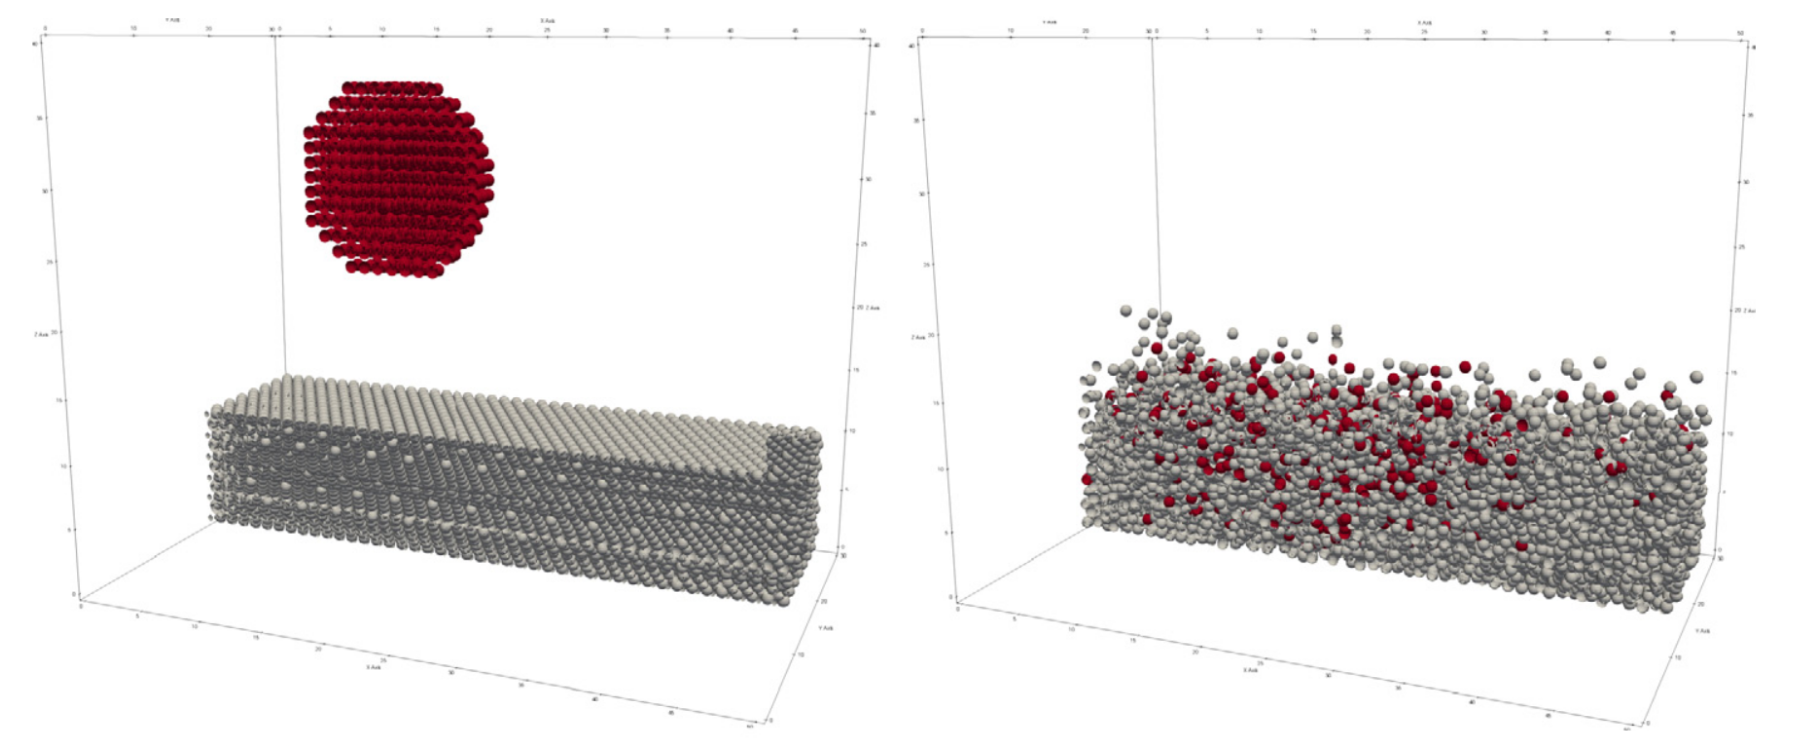
\includegraphics[width=0.9\linewidth]{imgs/fallingDrop.png} % Dynamically scale the image
    \captionof{figure}{Falling Drop \parencite{gratl2022n}}
    \label{fig:fd}
\end{minipage}%
\begin{minipage}[t]{0.5\textwidth} % Reserve half a row for the second picture
    \centering
    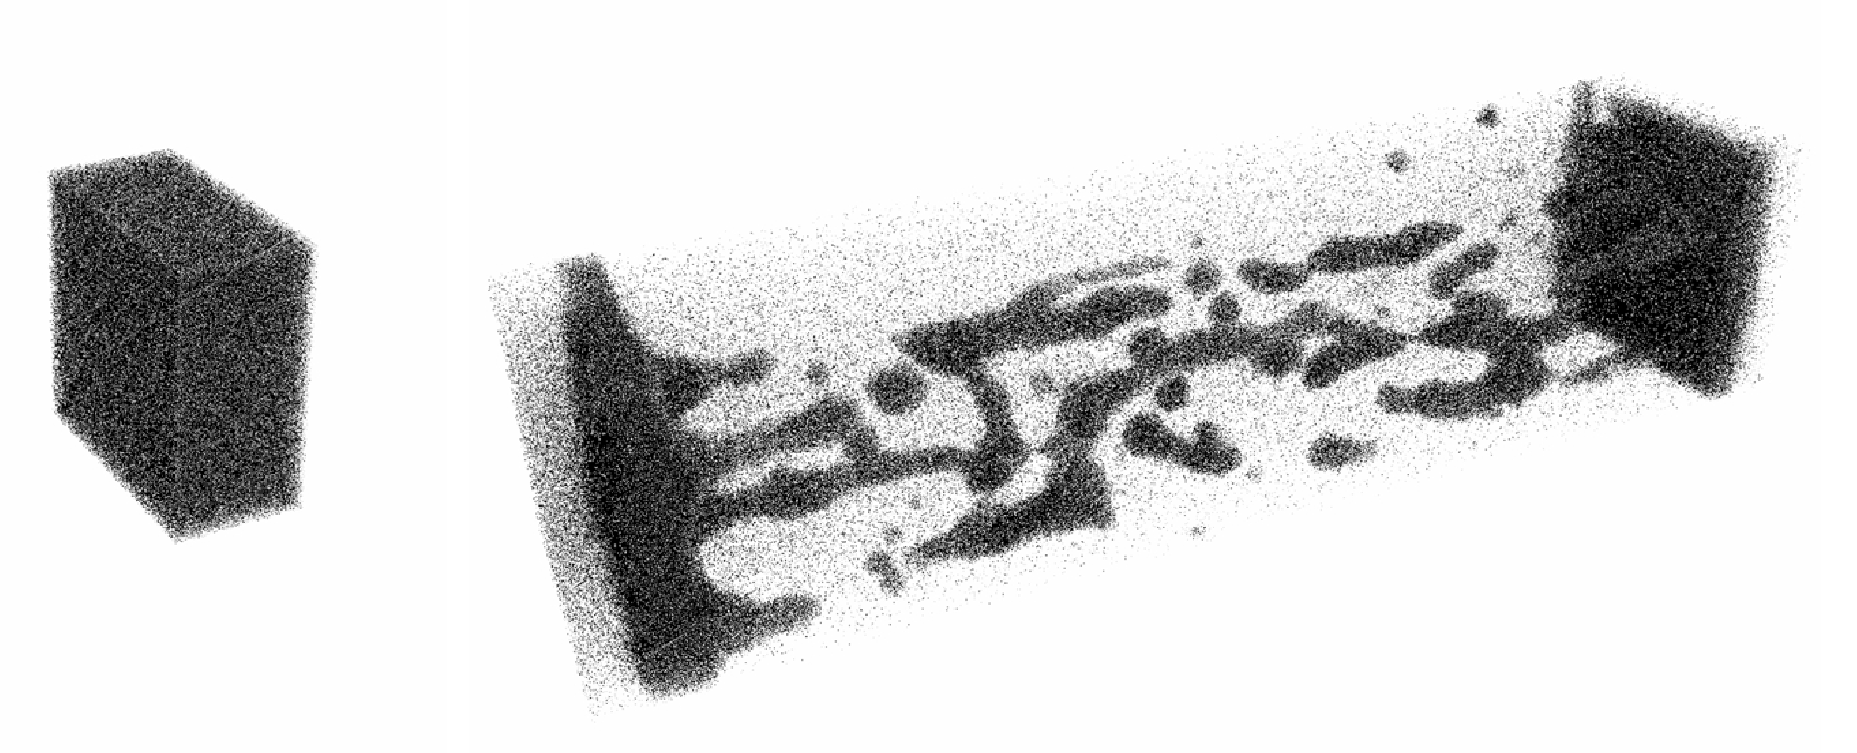
\includegraphics[width=0.9\linewidth]{imgs/explodingLiquid.png} % Dynamically scale the image
    \captionof{figure}{Exploding Liquid \parencite{seckler2021autopas}}
    \label{fig:exl}
\end{minipage}

\vspace{1em} % Optional vertical space between rows

\noindent
\begin{minipage}[t]{0.5\textwidth} % Reserve half a row for the third picture
    \centering
    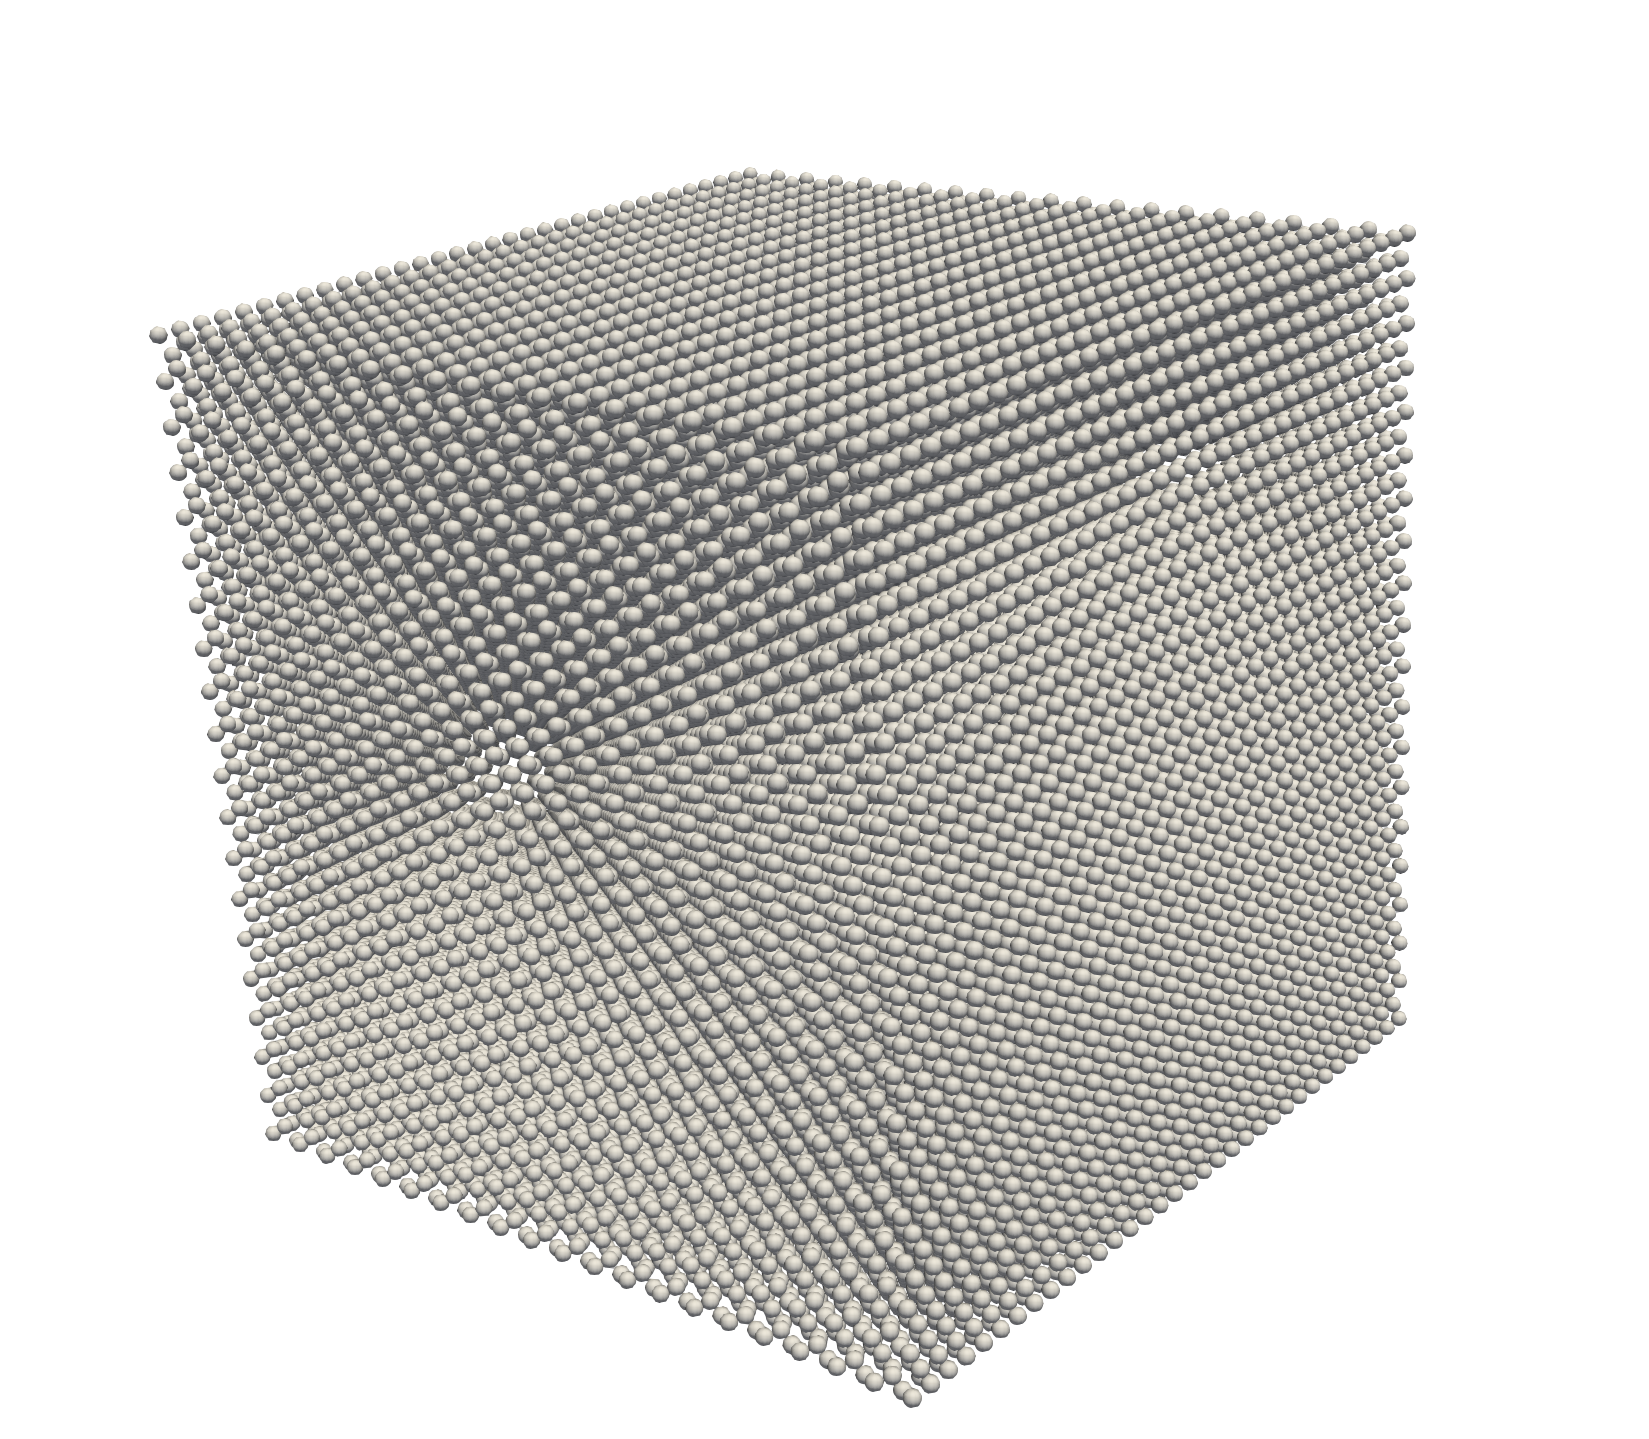
\includegraphics[width=0.5\linewidth]{imgs/constCube.png} % Dynamically scale the image
    \captionof{figure}{Constant Cube}
    \label{fig:conc}
\end{minipage}%
\begin{minipage}[t]{0.5\textwidth} % Reserve half a row for the fourth picture
    \centering
    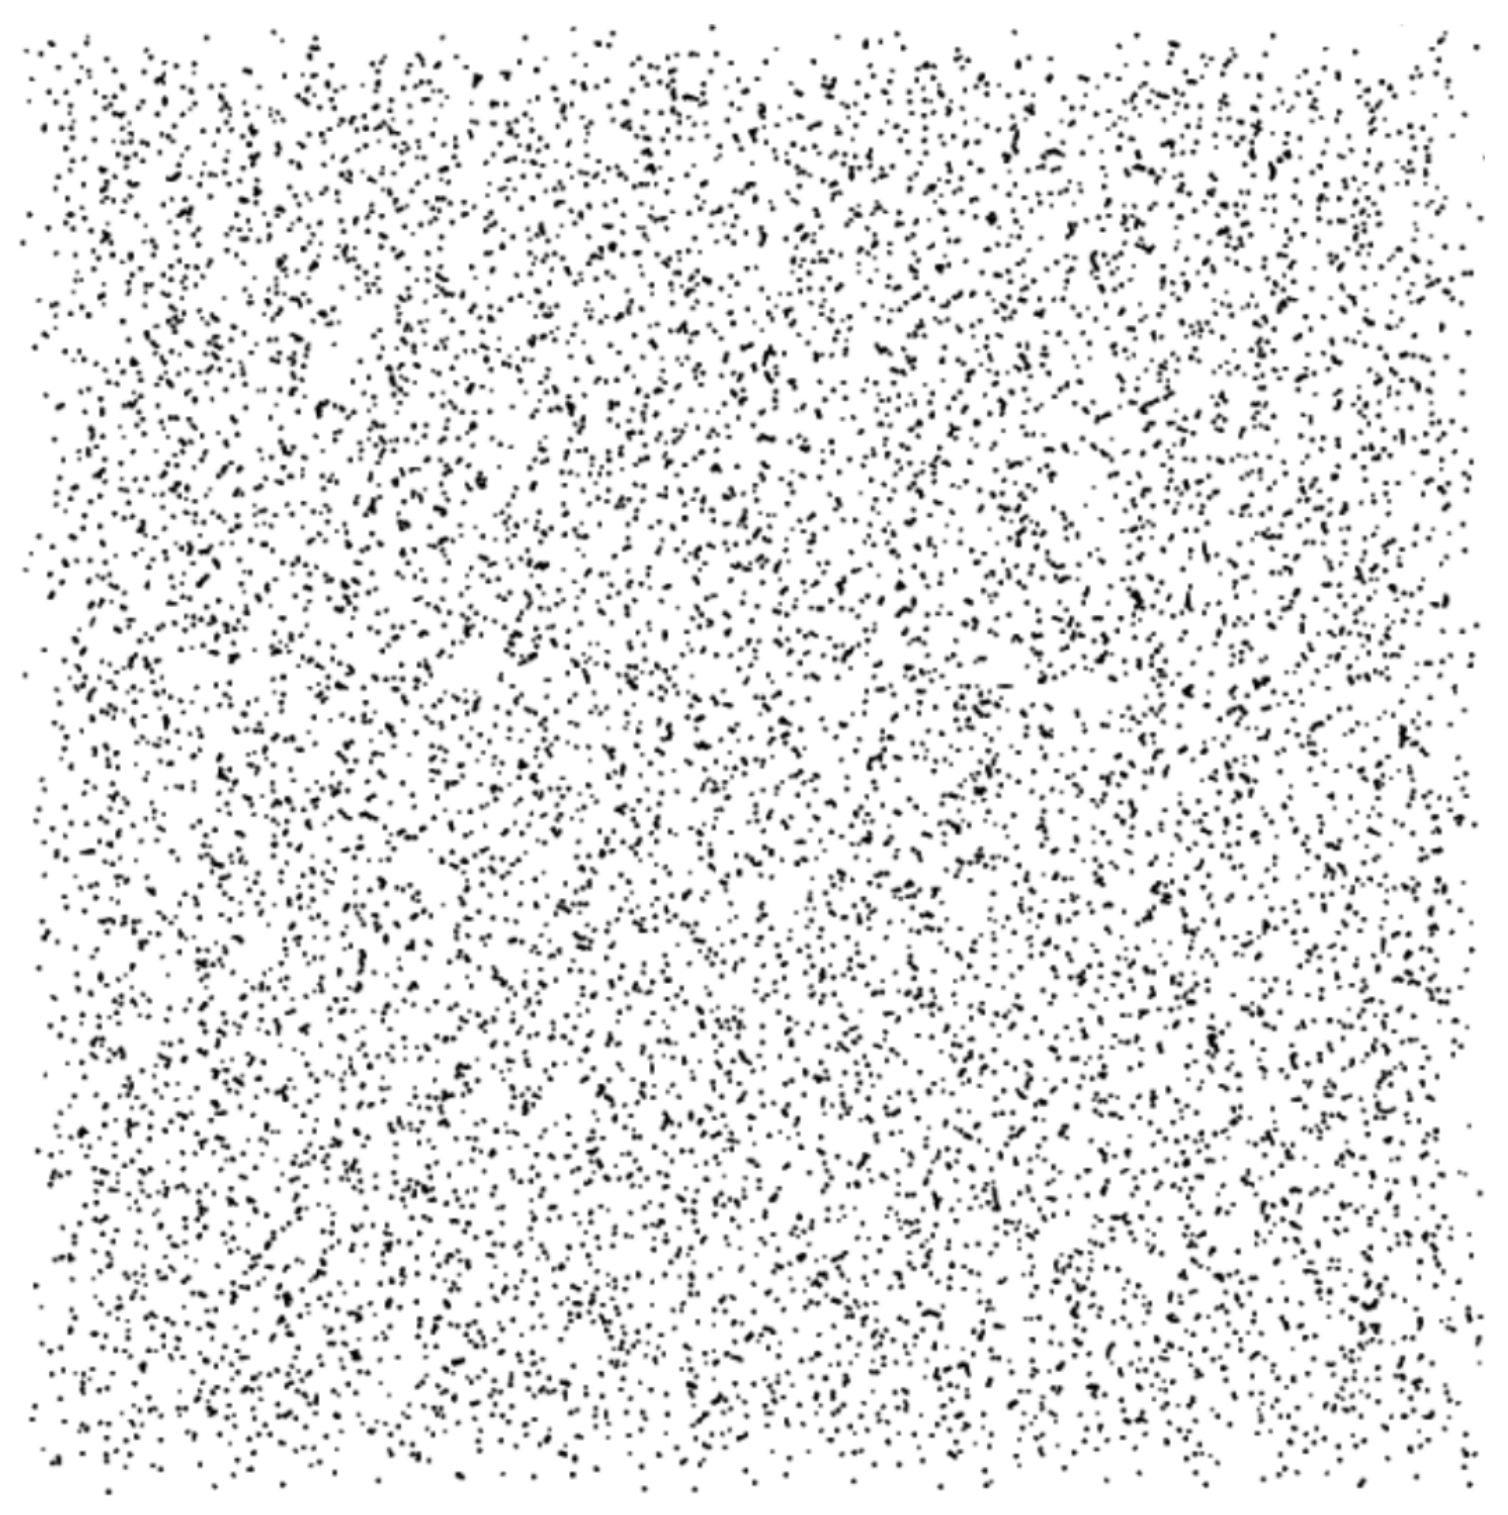
\includegraphics[width=0.5\linewidth]{imgs/spinodalDecomp.png} % Dynamically scale the image
    \captionof{figure}{Equilibration \parencite{Maximilian_Praus_Thesis-1.pdf}}
    \label{fig:equilibration}
\end{minipage}
\vspace{1em} 
\vspace{1em} 
\vspace{1em} 


% ======================================================================
\section{Results and Findings}


The primary objective was to evaluate the performance of the fast particle buffer by systematically modifying specific variables and observing its behavior across different scenarios. Additionally, the experiments aimed to assess the impact of these variables when applied in modified configurations of the same scenarios.

The variables selected for modification included:
\begin{itemize}
    \item \textbf{Verlet Rebuild Frequency}: This variable was adjusted to identify an optimal frequency that maximizes the reuse of neighbor lists across iterations without compromising runtime performance. The goal was to determine how much the rebuild frequency could be extended to achieve a performance gain.
    \item \textbf{Number of Particles}: Different simulation scenarios were selected, each with a varying number of particles, to examine how the buffer performs across different scales. The goal was to determine whether the buffer provides noticeable benefits in smaller simulations or if its advantages become more apparent in larger configurations.

    \item \textbf{Iteration Count}: By increasing the number of iterations, the experiments aimed to evaluate whether extending the runtime reduces the need for frequent neighbor list rebuilds in scenarios, where less fast particles are present after the dynamic phase.
\end{itemize}

The initial approach involved running a broad range of experiments, systematically varying these parameters to identify patterns and correlations. Key metrics of interest included the number of particles in the container versus the buffer and the time spent in \texttt{computeInteractions} compared to \texttt{remainderTraversal}. 
% The ultimate goal was to determine an ideal rebuild frequency and understand the relationship between these variables.

\subsection{Initial Test Series}

The initial series of experiments focused on analyzing frequency and iteration behavior across the first three scenarios. These experiments were run on CoolMUC2.

\subsubsection{Frequency Tests}

Frequency tests were conducted by varying the rebuild frequency between 10 and 15,810. The objective was to evaluate the runtime behavior for typical low frequencies and higher frequencies exceeding the total number of iterations (effectively disabling rebuilds apart from tuning). A logarithmic distribution of frequencies was chosen to emphasize the analysis of larger frequencies. The following Python function illustrates the frequency selection logic:

\begin{lstlisting}[style=mypython]
def get_step_size(freq):
    log_freq = math.log10(freq)
    step_diff = max_step - min_step
    step_size = min_step + (log_freq * step_diff / math.log10(end_freq))
    return int(step_size)
\end{lstlisting}

For each frequency experiment, four types of graphs were generated to help interpret the results more effectively:

\begin{enumerate}
    \item A frequency vs. runtime graph comparing the performance of the parent branch \texttt{DynamicVLMerge} with the \texttt{Fast Particle Buffer} branch.
    \item A graph highlighting the differences in \texttt{computeInteractions} runtime between the two branches.
    \item A graph illustrating the differences in \texttt{remainderTraversal}.
\end{enumerate}

The results consistently showed that the fast particle buffer performed worse across all scenarios and frequencies:
\begin{itemize}
    \item For the Falling Drop scenario, the runtime ranged from 1.1 to 6 times slower (Fig.\ref{fig:tuningfallingDrop}).
    \item For the Exploding Liquid scenario, the runtime ranged from 1.1 to 4 times slower (Fig.\ref{fig:tuningexplodingLiquid}).
    \item For the Constant Velocity Cube scenario, the runtime ranged from 1.3 to 11.2 times slower (Fig.\ref{fig:tuningconstantVelocityCube}).
\end{itemize}

To investigate the cause of this performance degradation, the focus was shifted to analyzing the graphs highlighting computeInteractions and remainderTraversal. However, these graphs were challenging to interpret due to significant spikes caused by the tuning phase. Tuning is the most computationally expensive part of the simulation, and its periodic spikes (determined by the tuning frequency) overshadowed the subtler runtime variations, making it difficult to analyze the true behavior of the buffer.


\begin{figure}[htbp]
    \centering
    \vspace{-0.5em}
    \begin{subfigure}[b]{\textwidth}
        \centering
        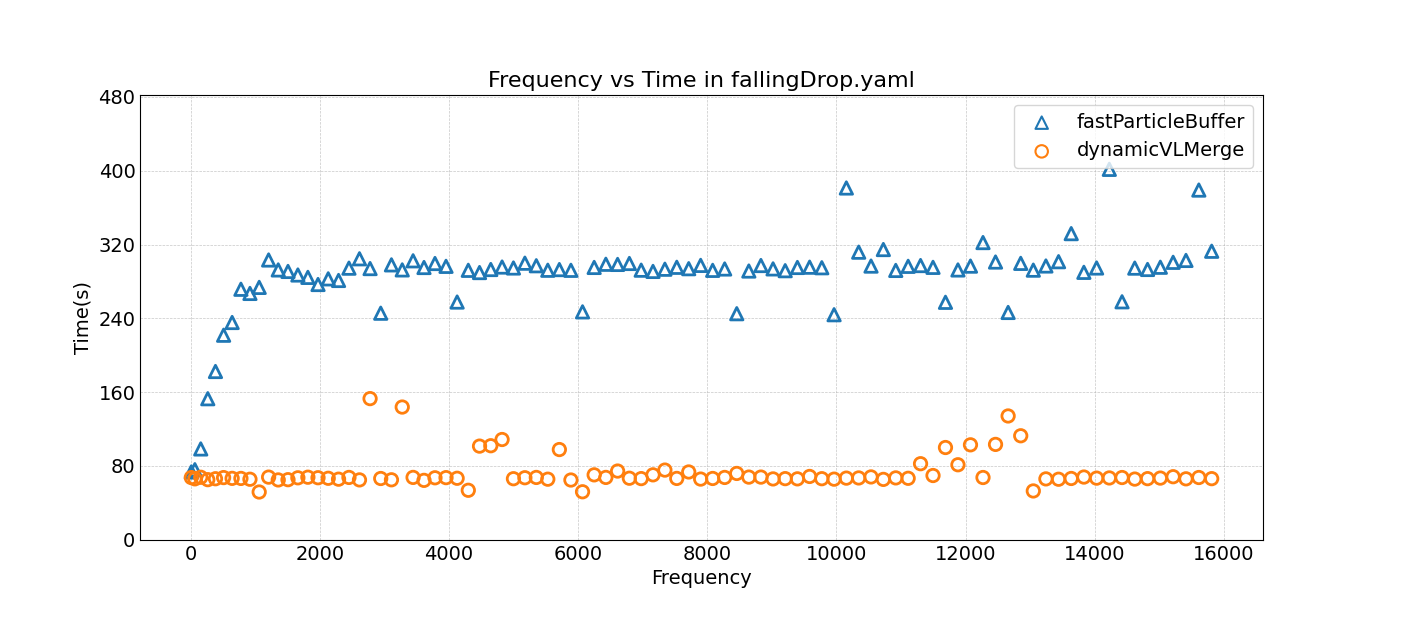
\includegraphics[width=0.9\linewidth]{graphs/fallingDrop/freqvstime.png}
        \vspace{-0.5em}
        \caption{\scriptsize Falling Drop}
        \label{fig:tuningfallingDrop}
    \end{subfigure}

    \begin{subfigure}[b]{\textwidth}
        \centering
        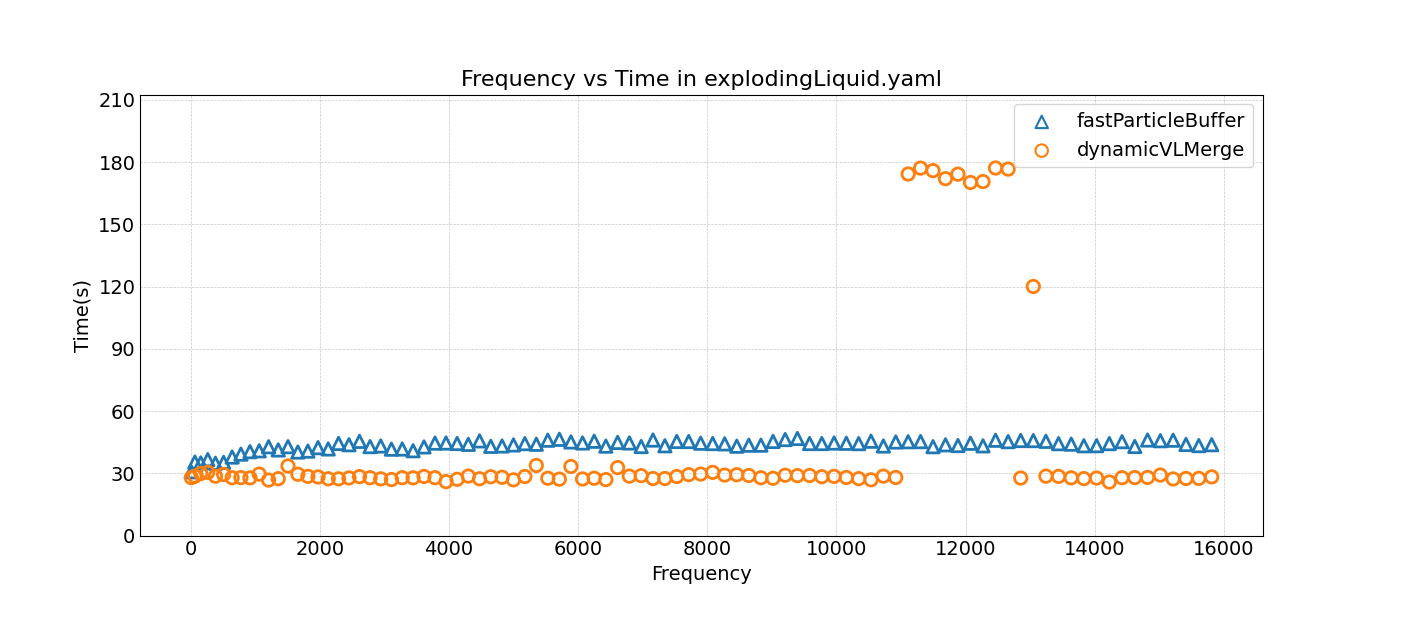
\includegraphics[width=0.9\linewidth]{graphs/explodingLiquid/freqvstime.png}
        \vspace{-0.5em}
        \caption{\scriptsize Exploding Liquid}
        \label{fig:tuningexplodingLiquid}
    \end{subfigure}

    \begin{subfigure}[b]{\textwidth}
        \centering
        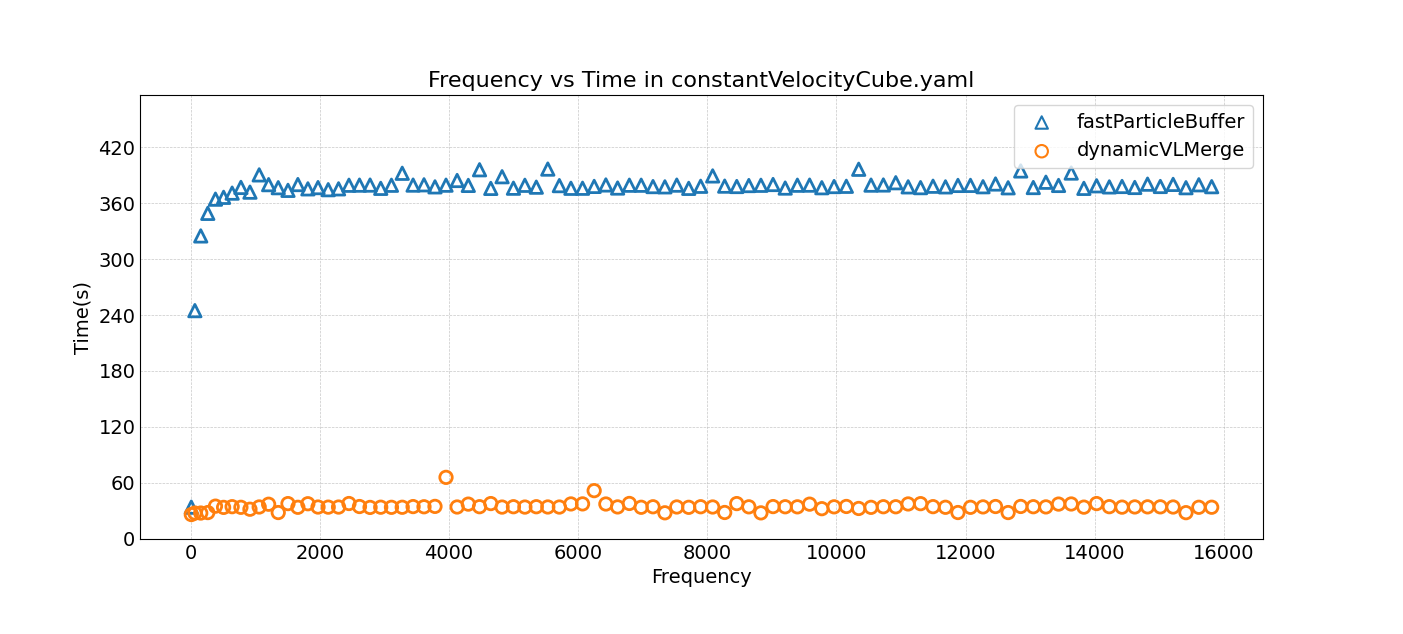
\includegraphics[width=0.9\linewidth]{graphs/constantVelocityCube/freqvstime.png}
        \vspace{-0.5em}
        \caption{\scriptsize Constant Velocity Cube}
        \label{fig:tuningconstantVelocityCube}
    \end{subfigure}

    \vspace{1em}
    \caption{Comparison of Frequency vs Time with Tuning}
    \label{fig:main}
\end{figure}



\subsubsection{Refined Tests Without Tuning}

To better understand the program's behavior, the tuning phase was effectively eliminated by specifying exact configurations for the container and traversal. This ensured that the simulation used fixed setups without requiring tuning. Since testing all possible configurations was impractical, three key traversal-container combinations were selected:


\begin{itemize}
    \item \textbf{Traversal}: \texttt{vlc\_c08 / vlp\_c08}, \textbf{Container}: VerletListsCells, \textbf{Data Layout}: AoS, \\ \textbf{Newton3}: Enabled
    \item \textbf{Traversal}: \texttt{vcl\_c06}, \textbf{Container}: VerletClusterLists, \textbf{Data Layout}: AoS, \\ \textbf{Newton3}: Enabled
    \item \textbf{Traversal}: \texttt{lc\_c08}, \textbf{Container}: LinkedCellsReferences, \textbf{Data Layout}: SoA, \\ \textbf{Newton3}: Enabled
\end{itemize}



Frequency tests were then repeated for the first three scenarios using these fixed configurations. This approach eliminated tuning-related noise, allowing for a clearer analysis of how the buffer performed under different traversal and container setups. By isolating these configurations, it was possible to focus on the individual behaviors of each traversal and container, leading to more thorough insights into the implementation's performance.

Upon examining the individual frequency versus time graphs, that compare the different configurations across various scenarios (Figures \ref{fig:mainFallingDrop} \ref{fig:mainExplodingLiquid} \ref{fig:mainConstantVelocityCube}), the implementation with the fast particle buffer generally underperformed relative to the implementation without it.

A unique case, however, is observed at frequency 10, where the Fast-Particle-Buffer branch performs nearly as well as the parent branch. This behavior occurs because, at such a low frequency, there are almost no fast particles; the neighbor lists are rebuilt so frequently that particles do not have sufficient time to accumulate in the buffer. 


\paragraph{Falling Drop:}

The runtime of the Fast-Particle-Buffer branch across all configurations was up to four times longer than that of the parent branch, Dynamic-VL-Merge (see Figure \ref{fig:mainFallingDrop}). This raises the question: what is the underlying cause of this difference in performance? 

To investigate, we focus on the relationship between  compute interactions, remainder traversal (Figure \ref{fig:vlcc08inter156}), and neighbor list rebuild times per iteration (Figure \ref{fig:vlcc08_neighbour_156}), as well as the number of particles stored in the buffer per iteration (Figure \ref{fig:vlcc08_buffer_size_156}).



\begin{figure}[htbp]
    \centering
    % \vspace{-0.5em}
    % \begin{subfigure}[b]{\textwidth}
        % \centering
        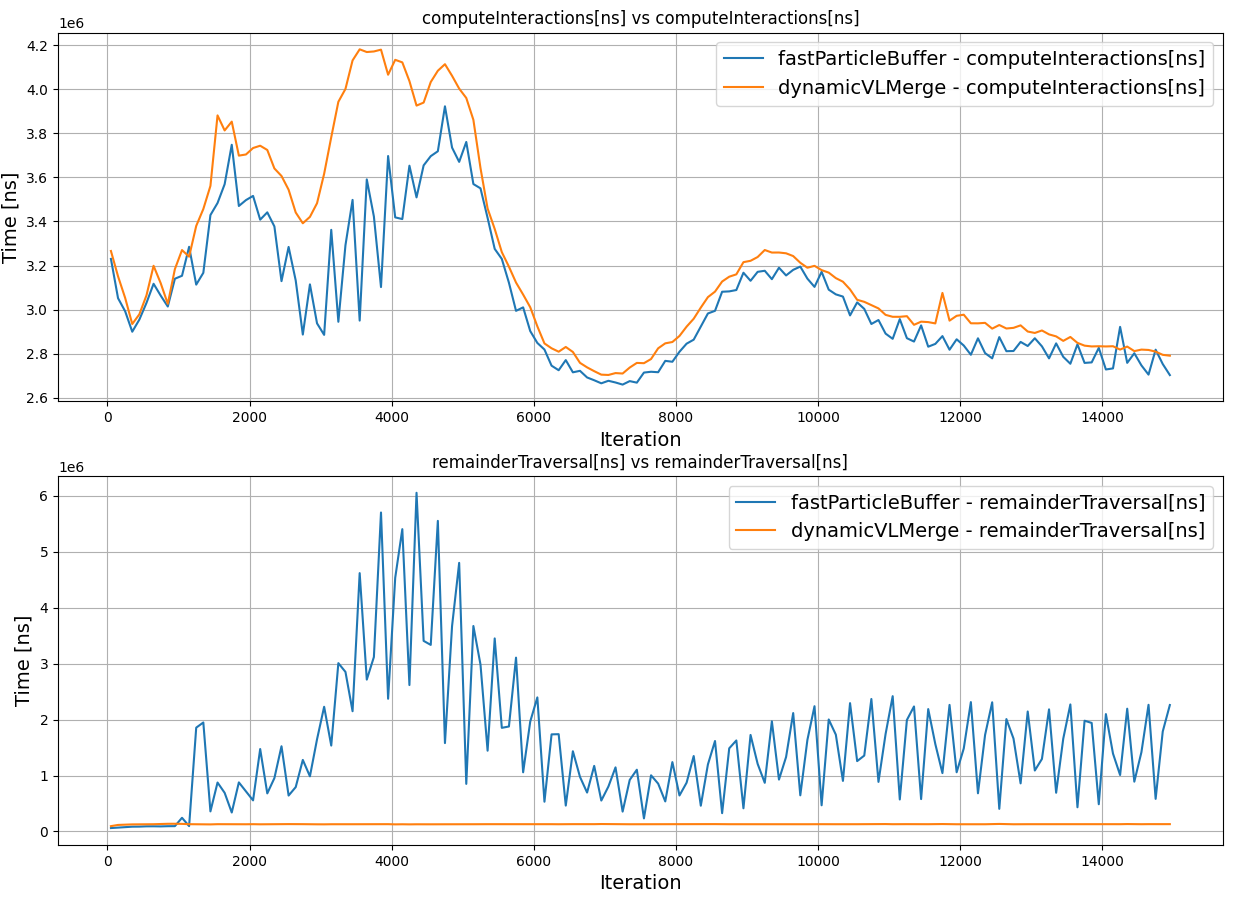
\includegraphics[width=0.9\linewidth]{graphs/fallingDrop/normalExperiments/freq/vlcc08inter156.png}
        \vspace{-0.5em}
        \caption{Compute interactions vs. remainder traversal in Falling Drop (vlc\_c08)}
        \label{fig:vlcc08inter156}
\end{figure}

\begin{figure}[htbp]
    \centering
    % \vspace{-0.5em}
    % \begin{subfigure}[b]{\textwidth}
        % \centering
        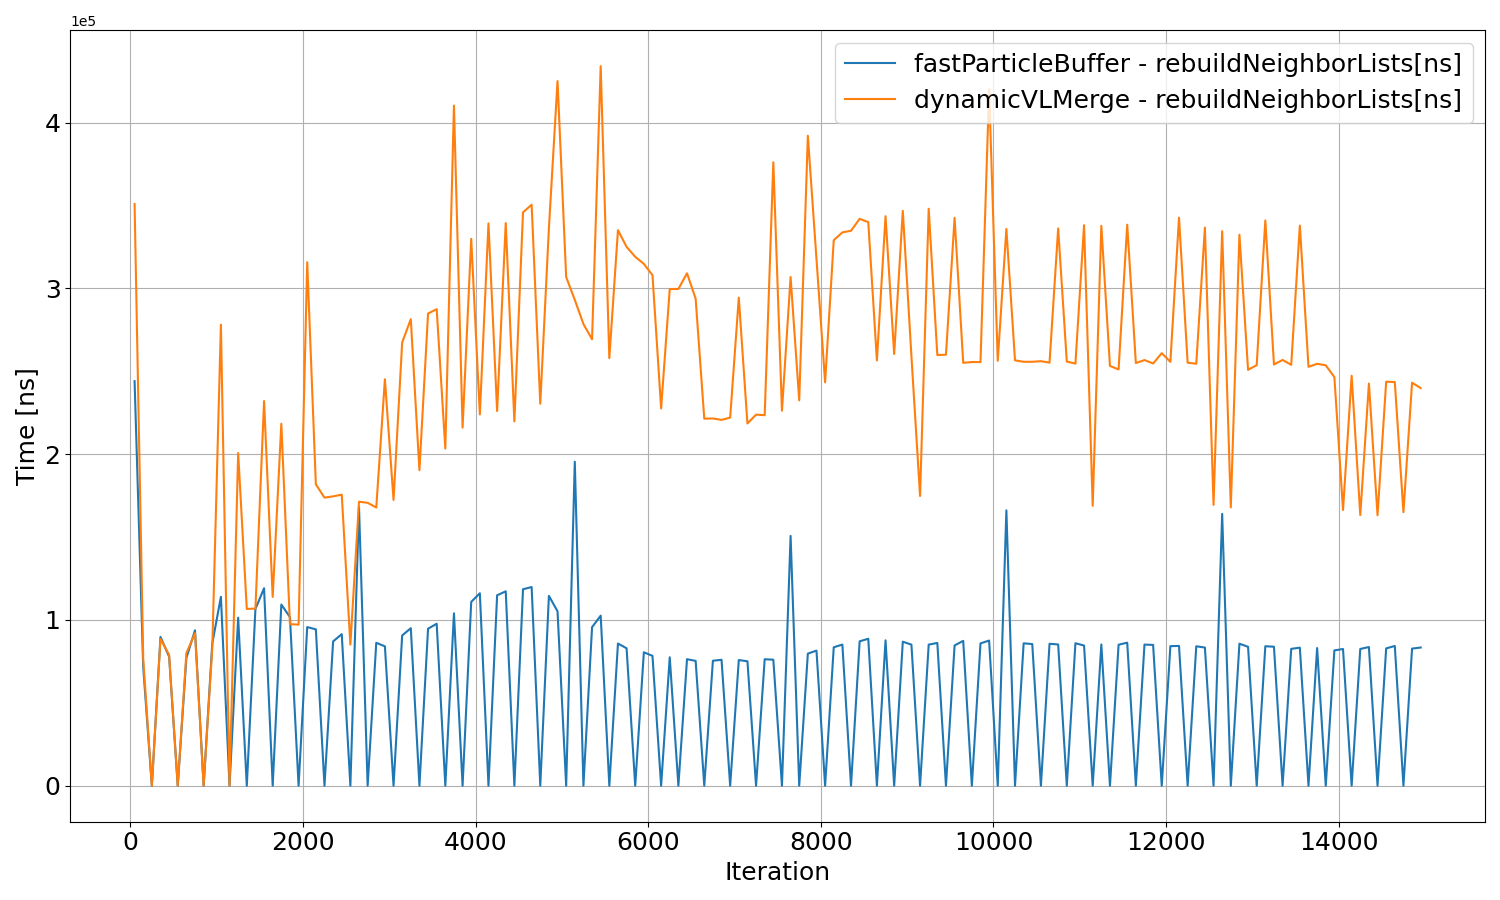
\includegraphics[width=0.9\linewidth]{graphs/fallingDrop/normalExperiments/freq/vlcc08_neighbour_156.png}
        \vspace{-0.5em}
        \caption{Time spent on neighbor list rebuilds in Falling Drop (vlc\_c08)}
        \label{fig:vlcc08_neighbour_156}
\end{figure}

\begin{figure}[htbp]
    \centering
    % \vspace{-0.5em}
    % \begin{subfigure}[b]{\textwidth}
        % \centering
        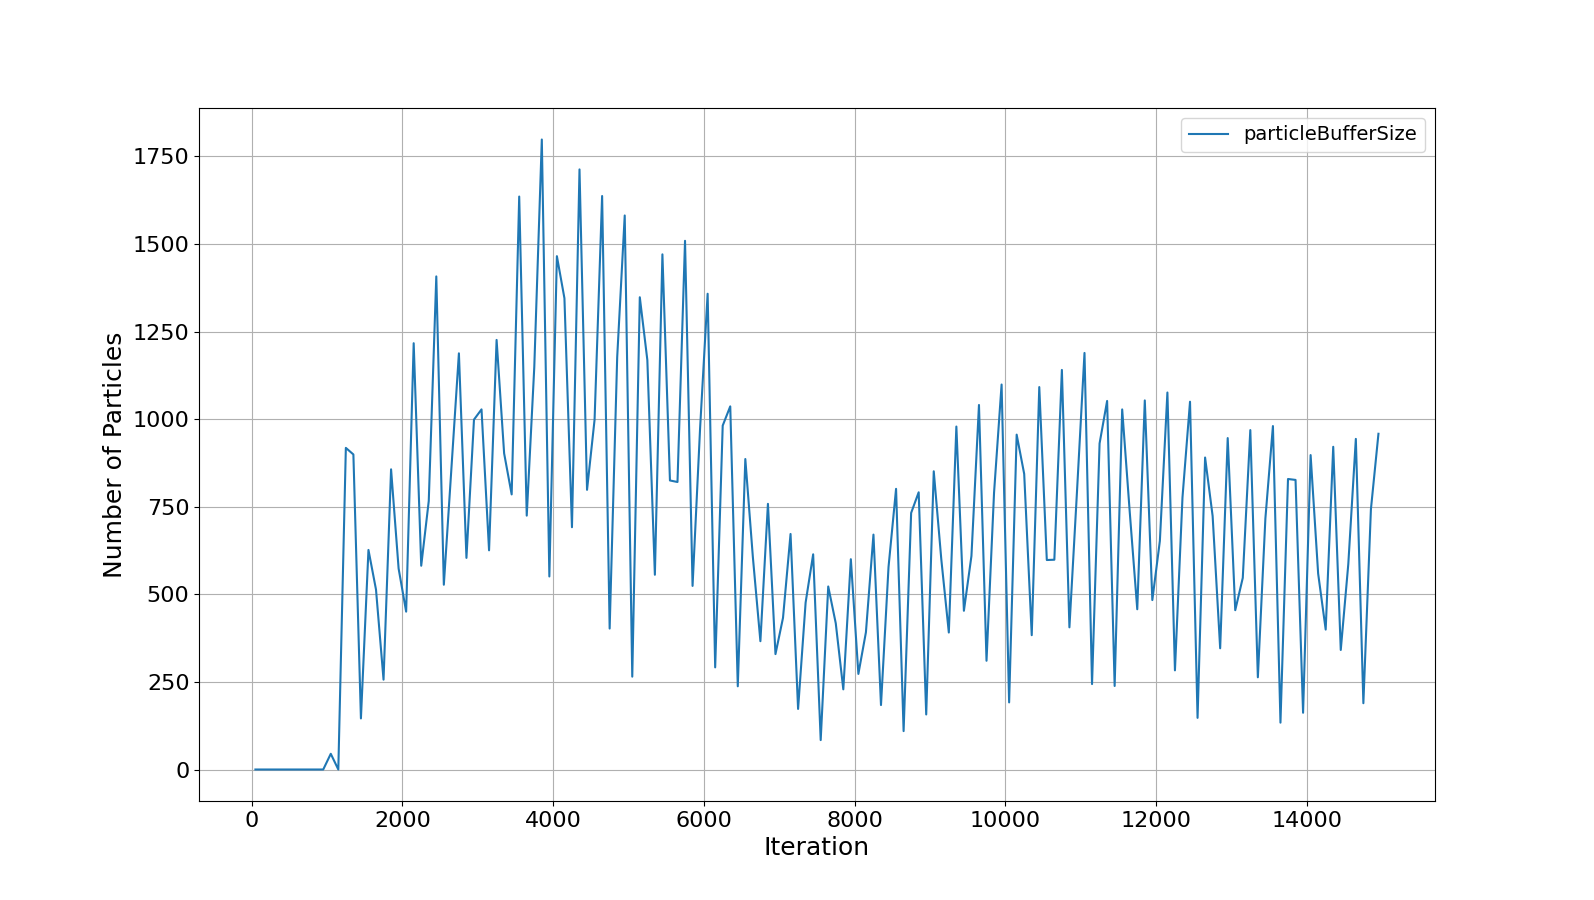
\includegraphics[width=\linewidth]{graphs/fallingDrop/normalExperiments/freq/vlcc08_buffer_size_156.png}
        \vspace{-0.5em}

        \caption{Buffer size over iterations in Falling Drop (vlc\_c08)}
        \label{fig:vlcc08_buffer_size_156}
\end{figure}



Between iterations 2000 and 5000, there is a gradual accumulation of particles in the buffer, peaking at approximately 1798 particles around iteration 3850. Following this peak, the number of particles in the buffer starts to decline. This fluctuation is directly reflected in the remainder traversal time, which increases as the buffer fills up and decreases once particles start leaving the buffer. 

While there is a reduction in the time spent on \texttt{computeInteractions} within the Fast-Particle-Buffer branch (due to particles being removed from the container), this saving is overshadowed by the significant increase in the time required for remainder traversal calculations. At its peak, the remainder traversal phase in the Fast-Particle-Buffer branch takes more time than the \texttt{computeInteractions} phase itself in the Dynamic-VL-Merge branch, where all particles are being considered. 

One noticeable advantage of the Fast-Particle-Buffer approach is the reduction in neighbor list rebuild time, which takes an average four times less time compared to the Dynamic-VL-Merge branch (Figure \ref{fig:vlcc08_neighbour_156}). However, the saved time does not compensate for the excessive time spent in remainder traversal. The combined savings from both reduced \texttt{computeInteractions} and neighbor list rebuilds are significantly smaller than the additional time required for remainder traversal.

At the end of the experiment, the recorded execution times for key operations in both branches are as follows:

\begin{itemize}
    \item \textbf{Fast-Particle-Buffer:}
    \begin{itemize}
        \item \texttt{computeInteractions[ns]}: $45.74$ s
        \item \texttt{remainderTraversal[ns]}: $23.40$ s
        \item \texttt{rebuildNeighborLists[ns]}: $0.92$ s
    \end{itemize}
    \item \textbf{Dynamic-VL-Merge:}
    \begin{itemize}
        \item \texttt{computeInteractions[ns]}: $48.23$ s
        \item \texttt{remainderTraversal[ns]}: $1.95$ s
        \item \texttt{rebuildNeighborLists[ns]}: $3.73$ s
    \end{itemize}
\end{itemize}

The higher the frequency, the more time is saved from avoiding neighbor list rebuilds. However, the rate at which remainder traversal time increases significantly outweighs the benefits. To illustrate, at frequency 15,810 (where rebuilding no longer occurs, as all particles are in the buffer), the theoretical maximum time savings from avoiding rebuilds is approximately $3.5 \times 10^5$ ns per iteration. However, the average remainder traversal time per iteration reaches approximately $1.38 \times 10^7$ ns, demonstrating that the overhead introduced by the buffer is vastly greater than the savings obtained from eliminating neighbor list rebuilds.

\paragraph{Constant Velocity Cube:}

This scenario exhibited similar behavior, where the fast particle buffer consistently underperformed compared to the counterpart (Figure \ref{fig:mainConstantVelocityCube}). Performance differences ranged from:
\begin{itemize}
    \item 6 times slower for \texttt{vlp\_c08} (selected instead of \texttt{vlc\_c08}, as \texttt{vlp\_c08} was frequently chosen during tuning experiments due to its optimization for this scenario).
    \item Up to 18 times slower for \texttt{lc\_c08}.
    \item Approximately 4 times slower for \texttt{vcl\_c06}.
\end{itemize}

The reasoning for these results remains consistent: the time saved from infrequent neighbor list rebuilds is outweighed by the excessive computation time in remainder traversals.

\paragraph{Exploding Liquid:} \label{para:exploding_liquid}
In the Exploding Liquid scenario, the traversals \texttt{lc\_c08} and \texttt{vlc\_c08} demonstrated similar performance trends to those observed in other scenarios (Figure \ref{fig:mainExplodingLiquid}). However, an exception was noted in the \texttt{vcl\_c06} traversal (Figure \ref{fig:vclc06explodingLiquid}). During this traversal, the Dynamic-VL-Merge branch exhibited an average runtime nearly twice as long as the other two traversals, whereas the runtime of the Fast-Particle-Buffer branch increased only slightly in comparison.

Analyzing frequencies between 10 and 2451, the Fast-Particle-Buffer branch outperformed the Dynamic-VL-Merge branch. The shortest runtime achieved by the Fast-Particle-Buffer branch was 37.88 seconds at frequency 265, whereas the lowest runtime for the Dynamic-VL-Merge branch within \texttt{vcl\_c06} was 39.2 seconds in iteration 9963. 


A deeper analysis of the \texttt{computeInteractions} and \texttt{remainderTraversal} times provides insight into the underlying reason for this speedup. Unlike in other traversals, \texttt{computeInteractions} in the parent branch consumed significantly more time using \texttt{vcl\_c06}, whereas the remainder traversal time in the Fast-Particle-Buffer branch experienced changes that were not as drastic (Fig. \ref{fig:mainexplodingLiquid_inter}). This discrepancy led to a unique case where the increased computational cost of \texttt{computeInteractions} in the Dynamic-VL-Merge branch effectively offset the additional remainder traversal time in the Fast-Particle-Buffer branch. Consequently, for \texttt{vcl\_c06}, the Fast-Particle-Buffer branch gained a net advantage by reducing the cost of neighbor list rebuilds.

However, while this might initially appear as a speedup, it is important to put the results into context. The lowest overall runtime across all traversal methods was not achieved by the Fast-Particle-Buffer branch but rather by the Dynamic-VL-Merge branch in other traversal configurations. This suggests that, although the Fast-Particle-Buffer branch outperformed the Dynamic-VL-Merge branch specifically for \texttt{vcl\_c06}, it was not the most efficient approach across all tested traversal methods. Therefore, while the buffer mechanism provided a performance gain in this isolated case, it did not lead to an overall improvement in execution time across the entire experiment.




\subsubsection{Iteration Tests}


For the iteration tests, a base frequency of 100 was maintained for the first two scenarios and 1000 for the third scenario. The number of iterations varied between 500 and 30,000, with a step size of 500 iterations. The goal of these experiments was to observe the behavior of fast particles at different stages of the simulation by increasing the number of iterations. This approach aimed to identify any correlations between simulation progression and the performance of the particle buffer implementation, as well as to expand the range of experiments conducted.

Initially, as in the frequency tests, the first three scenarios were executed with tuning enabled. However, as earlier this approach did not give us a clear enough understanding of the performance of the fast particle branch. The results of these initial tests are presented in Figurev\ref{fig:mainIterWithTuning}.

\subsubsection{Individual Test Results}

\textbf{Falling Drop Scenario:}
For the \texttt{vlc\_c08} traversal, no performance improvement was observed. Across all iteration counts, the fast particle buffer consistently performed worse than the Dynamic-VL-Merge branch. 

The same trend was observed for \texttt{lc\_c08}. The remainder traversal phase required excessive time, negating any potential gains from avoiding neighbor list rebuilds. Thus, the time saved from fewer rebuilds was insufficient to offset the overhead introduced by the remainder traversal.


On the other hand, the \texttt{vcl\_c06} traversal displayed similar performance in both branches, with the fast particle buffer occasionally running 1-2 seconds faster. This behavior follows the same reasoning as in \ref{para:exploding_liquid}, that being the pronounced increase in runtime for \texttt{computeInteractions}. Specifically, for \texttt{vcl\_c06}, \texttt{computeInteractions} required nearly four times more runtime than in \texttt{vcl\_c08}. While the fast particle buffer also experienced a runtime increase, it was less pronounced than in the Dynamic-VL-Merge, explaining why the overall performance remained similar. While these results suggest some efficiency gains in this particular experiment, they do not indicate a significant overall performance improvement. The corresponding plots can be found in \ref{fig:mainfallingDropIter}.


\textbf{Exploding Liquid Scenario:}
The results for this scenario followed a pattern similar to Falling Drop. However, anomalies were observed in the behavior of \texttt{vlc\_c08} and \texttt{vcl\_c06}, as indicated in Figure \ref{fig:mainexplodingLiquidIter}. Missing plotting points in the graphs suggest that the experiment failed for certain iteration counts in both branches. Although there were spikes in \texttt{vlc\_c08} (Figure \ref{fig:vlcc08explodingLiquidIter}), where the fast particle buffer branch appeared to outperform the Dynamic-VL-Merge, the anomalies in the experiments make these results unreliable. The \texttt{lc\_c08} traversal exhibited stable behavior with no failed runs; however, the results were fairly routine and did not provide significant new insights into the topic.


\textbf{Constant Velocity Cube Scenario:}
In this scenario, no performance improvement was observed for the fast particle buffer. Instead, the performance difference between the two branches was more pronounced compared to Falling Drop. For \texttt{lc\_c08}, the fast particle buffer was up to 16 times slower; for \texttt{vcl\_c06}, it was 4 times slower; and for \texttt{vlp\_c08}, it was around 3 times slower.
This poor performance is due to the large number of particles accumulating in the buffer. For instance, in the experiment with 30,000 iterations, more than half of the total particles—around 28,000 out of 50,000—were in the buffer. This high number of particles in the buffer significantly increased the time required for remainder traversal. This is illustrated in Figure ~\ref{fig:fpbvsdvl_vlpc08}, where the runtime scale for the remainder traversal is $e8$, while \texttt{computeInteractions} operates on the $e7$ scale, highlighting a clear difference in time consumption.

% The issue lies in the difference in optimization between the buffer and the container. Containers and traversals are designed to be efficient and parallelized, allowing particles to be processed quickly. In contrast, the fast particle buffer is a simple vector of vectors and is not optimized in the same way, leading to much higher computation times for remainder traversal when many particles are stored in the buffer.


\begin{center}
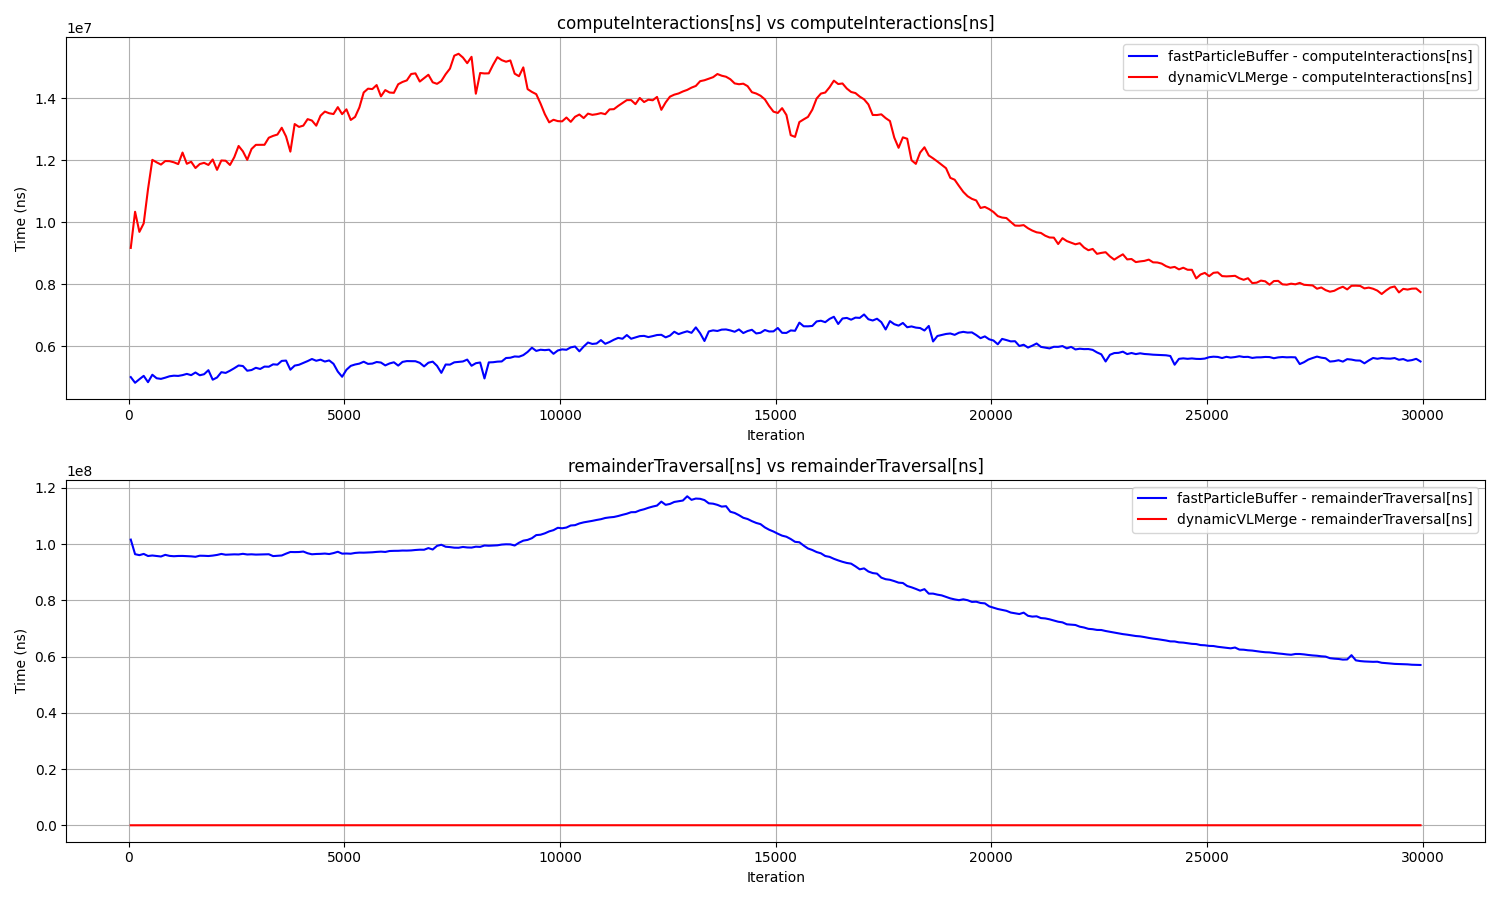
\includegraphics[width=\linewidth]{graphs/constantVelocityCube/normalExperiments/iter/vlpc08dvlpb.png}
\captionof{figure}{Compute Interactions vs Remainder Traversal in Constant Velocity Cube (vlp\_c08)}
\label{fig:fpbvsdvl_vlpc08}
\end{center}




% percentage expr
%     - why only run in some of them
%     - why still not performat
%     - why chose to use spinodal all of a sudden 
%     - idea to converge to DVL
%     - is the slight improvement only a coincidence - repeating the tests many times
%     - idea to increase the temperatur in spinodial decomp 
% Profiler
% add where to find the tests on github and such, also attach slurm job maybe


\subsection{Percentage Experiments}

The primary challenge with the fast particle buffer implementation is that the time required for \texttt{remainderTraversal} significantly outweighs the time saved from reducing the frequency of neighbor list rebuilds. To address this issue, a percentage-based threshold was introduced, limiting the number of particles that can accumulate in the buffer to a fixed percentage of the total number of particles in the container. The objective was to reduce the time spent in remainder traversal, while still benefiting from fewer neighbor list rebuilds.

Given that \texttt{rebuildFrequency} is directly tied to the particle buffer's efficiency, these experiments focus on adjusting the rebuild frequency rather than the number of iterations. In earlier experiments, the iteration count was varied to see how performance evolved over longer runtimes. However, since rebuild frequency determines when particles move in and out of the buffer, varying it gives a more precise understanding of the buffer's efficiency, making it the primary focus of this set of experiments.

Initially, experiments were conducted across frequencies ranging from 10 to 1900, based on the previous findings that smaller frequencies performed better. Threshold values of 10\%, 15\%, 20\%, and 30\% were tested, meaning that if the buffer contained the specified percentage of the container's particles, a rebuild was triggered.

For frequencies above 100, the performance gap between the Fast-Particle-Buffer branch and Dynamic-VL-Merge increased, with the latter performing better. However, for frequencies below 100, certain thresholds—particularly the 10\% threshold—showed slight performance improvements of a few seconds. The complete set of graphs supporting these findings is available in the provided \href{https://github.com/xhulia028/GraphView}{\texttt{repository}}.


To further analyze these trends, the Falling Drop scenario was selected as it displayed consistent behavior across different configurations. The traversal \texttt{vlc\_c08} was chosen as it was one of the better-performing traversals in previous experiments.


Given that performance improvements remained minor—mostly 1 to 2 seconds—the experiments were repeated four times per configuration to improve accuracy. Moreover, smaller threshold values were introduced:  
5\%, 1\%, 0.5\%, and 0.1\%, along with ultra-small thresholds of 0.01\%, 0.001\%, and 0\%, to analyze how performance evolves as the Fast-Particle-Buffer branch converges toward the Dynamic-VL-Merge branch. The primary goal of this extension was to confirm that any observed performance gains were genuinely due to the buffer mechanism.


The experimental data is presented as a box plot in Figure \ref{fig:percentage_falling}, where red dots represent the mean runtime for each experiment. Only frequencies from 20 to 300 are shown, as including all frequencies would make the graph appear too cluttered. However, these selected frequencies cover the main bulk of the data and are the most representative ones. The rest of the data can be found in the provided \href{https://github.com/xhulia028/GraphView}{\texttt{repository}}. The key findings are as follows:

\begin{itemize}
    \item On average, thresholds between 0.1\% and 1\% provided the best performance.
    \item Extremely small thresholds (0.01\%, 0.001\%, 0\%) sometimes performed worse than the Dynamic-VL-Merge branch. This can be explained by the overhead introduced by continuously scanning the container to check whether the threshold condition was met.
    \item Although some configurations achieved minor performance improvements, these gains were marginal and nearly insignificant compared to the overall runtime.
\end{itemize}



\begin{center}
    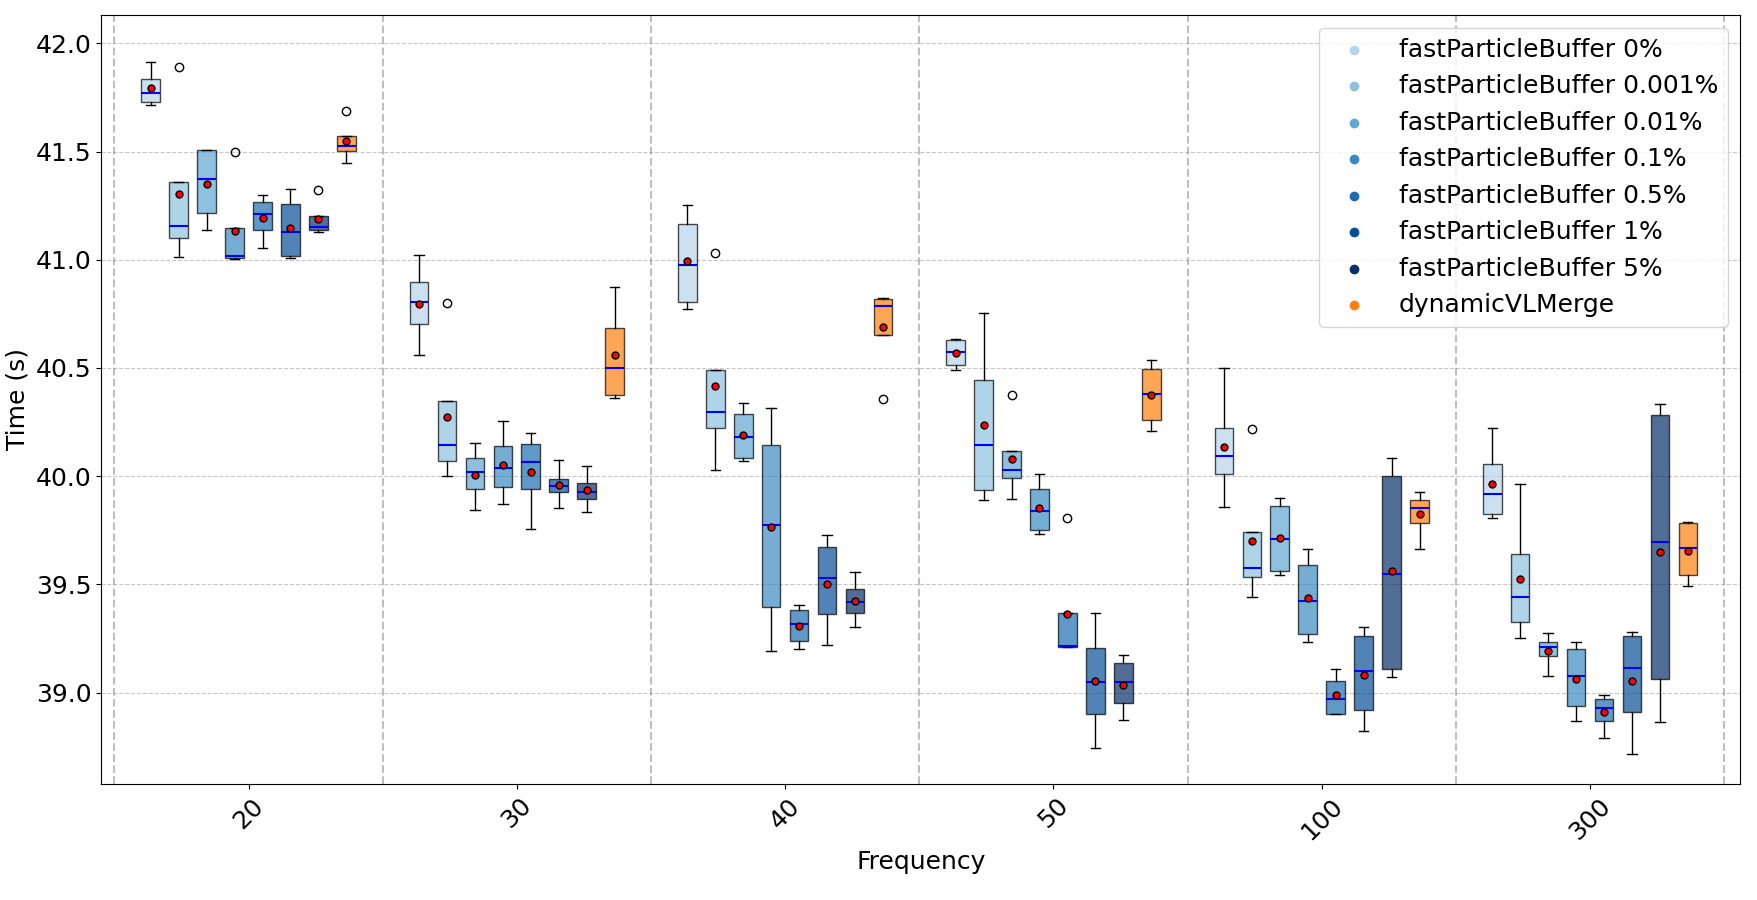
\includegraphics[width=\linewidth]{graphs/percentage_vlcc08.png}
    \captionof{figure}{Percentage Experiments in Falling Drop (vlc\_c08)}
    \label{fig:percentage_falling}
\end{center}



\subsection{Equilibration}
 
Based on the earlier experiments, the observed performance improvement was minimal, leading to the question of whether the selected test cases were limiting the analysis. Instead of focusing on short simulations lasting around a couple of minutes or less, a more dynamic scenario with a significantly larger number of particles was needed. For this reason, the equilibration scenario was chosen.

The hypothesis was that, due to its highly dynamic nature and large particle count (4 million), this scenario would be better suited to reveal potential performance benefits of the fast particle buffer.

From prior frequency experiments, it was observed that the particle buffer performed better at smaller frequencies. Therefore, this experiment focused on frequencies ranging from 10 to 50 with a step size of 10. Additionally, as established earlier, smaller thresholds tended to yield better results. Considering the large particle count in the equilibration scenario, initial tests were conducted with thresholds of 1\% and 5\% of the container's particles. 

It is important to note that 1\% and 5\% of 4 million correspond to 40,000 and 200,000 particles, respectively, which exceed the total particle count of the other scenarios.

\textbf{Results for \texttt{vlc\_c08}:}  
Throughout this scenario the average runtime for the Dynamic-VL-Merge branch consisted of 9 hours and 59 minutes (Figure \ref{fig:equ_normla_vlcc08}). When the threshold was set to 5\%, the fast particle buffer demonstrated a performance improvement of 4.2\% (equivalent to saving 25 minutes) at frequency 30. At frequency 20, the improvement was 2.5\% (saving 15 minutes). For frequency 10, the runtime was marginally worse by 1\%. However, for larger frequencies, such as 40 and 50, there was a significant slowdown of 44\% and 111\%, respectively.

For the 1\% threshold, fluctuations were less pronounced compared to the 5\% threshold. The runtime for all frequencies was closer to that of the Dynamic-VL-Merge branch. A performance improvement of 2.2\% (equivalent to 13 minutes) was observed at frequency 20, and 3\% (18 minutes) at frequency 30. For frequencies 10 and 50, the runtime was nearly identical to the parent branch, differing by only ±1 minute. At frequency 40, there was a minor slowdown of 1\% (6 minutes), which is relatively insignificant.

The fastest runtime in this experiment was achieved by the Fast-Particle-Buffer with a 5\% threshold at frequency 30, completing in 9 hours and 33 minutes. The second-fastest was the Fast-Particle-Buffer with a 1\% threshold, which took 6 minutes longer.

For the Dynamic-VL-Merge branch, the shortest runtime was 9 hours and 47 minutes, recorded at frequency 40. Comparing the best results from both approaches, the Fast-Particle-Buffer provided a speedup of 14 minutes, equivalent to a 2.74\% improvement over the fastest Dynamic-VL-Merge run.

\begin{center}
    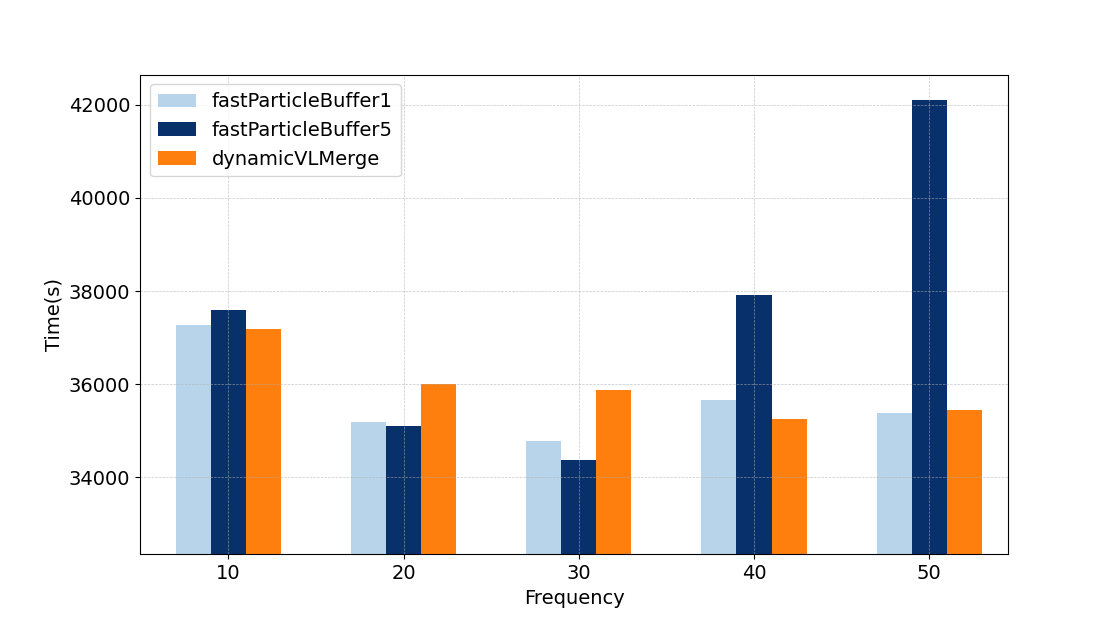
\includegraphics[width=0.8\linewidth]{graphs/spinodalDecomposition/vlcc08.png}
    \captionsetup{hypcap=false}
    \captionof{figure}{Frequency vs Time for Equilibration (vlc\_c08)}
    \label{fig:equ_normla_vlcc08}
\end{center}



\textbf{Results for \texttt{lc\_c08}:}  
Using LinkedCellsReferences with traversal \texttt{lc\_c08} (Figure \ref{fig:equ_normla_lcc08}), the average runtime for the Dynamic-VL-Merge branch was 14 hours and 27 minutes, approximately 4 hours and 30 minutes longer than the \texttt{vlc\_c08} configuration.

At a 5\% threshold, a 1.94\% performance improvement (16 minutes) was observed at frequency 30, with a smaller 0.9\% improvement (7 minutes) at frequency 20. However, for all other frequencies, no improvement was recorded. In contrast, at frequencies 40 and 50, the runtime of the Fast-Particle-Buffer branch increased significantly. At frequency 50, the performance degraded to the point where the simulation timed out.


For the 1\% threshold, a more notable improvement was observed at frequency 30, with a 2.3\% improvement (20 minutes). For the remaining frequencies, the runtime was very similar to the parent branch, fluctuating between -0.96\% and 0.29\% of the respective Dynamic-VL-Merge runtimes.

For this container-traversal combination, the fastest experiment overall was achieved using the Fast-Particle-Buffer with a 1\% threshold at frequency 30, resulting in a runtime of 14 hours and 4 minutes. This corresponds to a 12-minute improvement (1.43\%) compared to the Dynamic-VL-Merge branch at frequency 20, which recorded the fastest runtime for that branch.


\begin{center}
    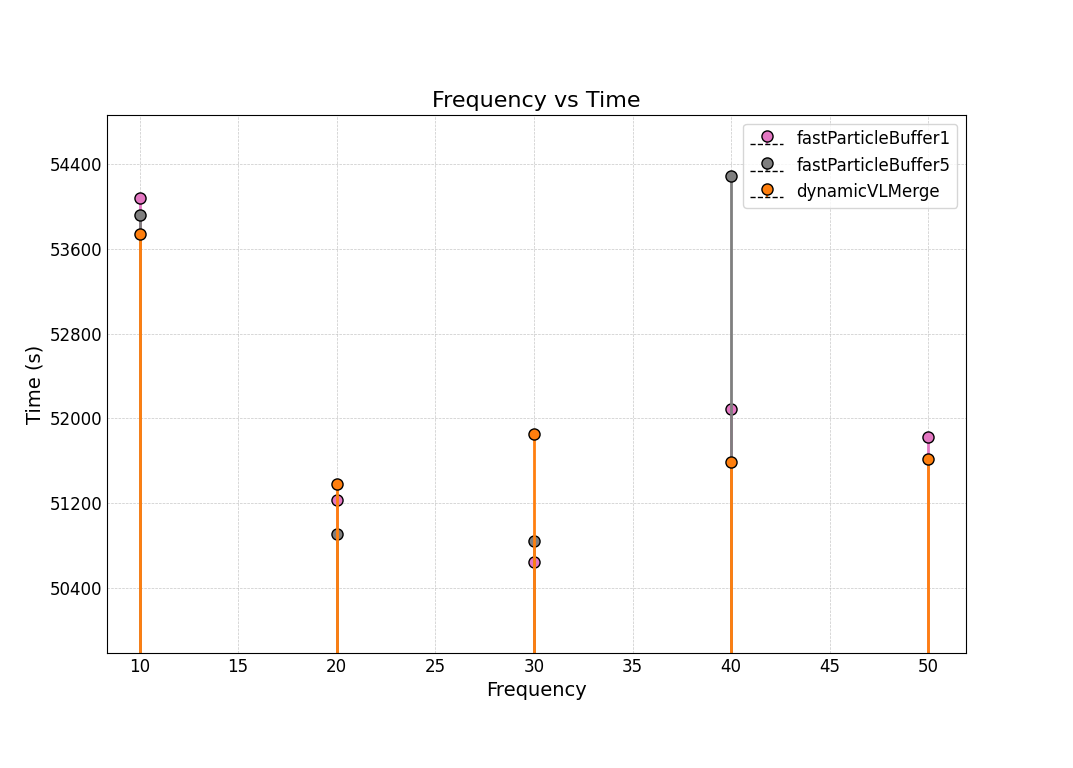
\includegraphics[width=0.8\linewidth]{graphs/spinodalDecomposition/lcc08.png}
    \captionsetup{hypcap=false}
    \captionof{figure}{Frequency vs Time for Equilibration (lc\_c08)}
    \label{fig:equ_normla_lcc08}
\end{center}
    
    

% \textbf{Summary:}  
% The results demonstrate that performance improvements using the fast particle buffer are highly scenario- and configuration-dependent. While significant speedups were observed at specific thresholds and frequencies, the benefits diminished or reversed at higher frequencies or with larger thresholds. The experiment highlights the importance of fine-tuning parameters to achieve optimal performance, especially in highly dynamic scenarios with large particle counts.


\subsubsection{Equilibration with Increased Temperature}

To further amplify the number of fast particles and make the experiment more dynamic, the temperature of the system in the equilibration scenario was increased. This adjustment resulted in molecules with higher kinetic energy, thereby increasing their speed. The focus of this experiment remained on the same frequencies as in previous tests, with the addition of a new frequency, 5, to further investigate performance trends at lower rebuild intervals. For this experiment, the \texttt{vlc\_c08} traversal configuration was used, as the \texttt{lc\_c08} configuration proved too inefficient, resulting in timeouts at the maximum allowed runtime of 16 hours.

In this configuration, the fast particle buffer with a threshold of 1\% achieved an 8.6\% performance improvement at frequency 10. This translates to a time saving of 60 minutes from a total runtime of 11 hours and 42 minutes. Similarly, the fast particle buffer with a threshold of 5\% exhibited a 7.8\% performance improvement at the same frequency, resulting in a 55-minute reduction from the same total runtime.

For the remaining frequencies, neither version of the fast particle buffer outperformed the Dynamic-VL-Merge branch. However, the overall fastest experiment was the Fast-Particle-Buffer with a 1\% threshold, achieving a 41-minute improvement compared to the fastest version of the Dynamic-VL-Merge branch at frequency 40. This corresponds to a 6\% performance boost, the largest improvement observed in the experiments so far. The results are summarized in Figure~\ref{fig:equilibration_plot_increased_temp}, which visualizes the performance trends across different configurations.

\begin{center}
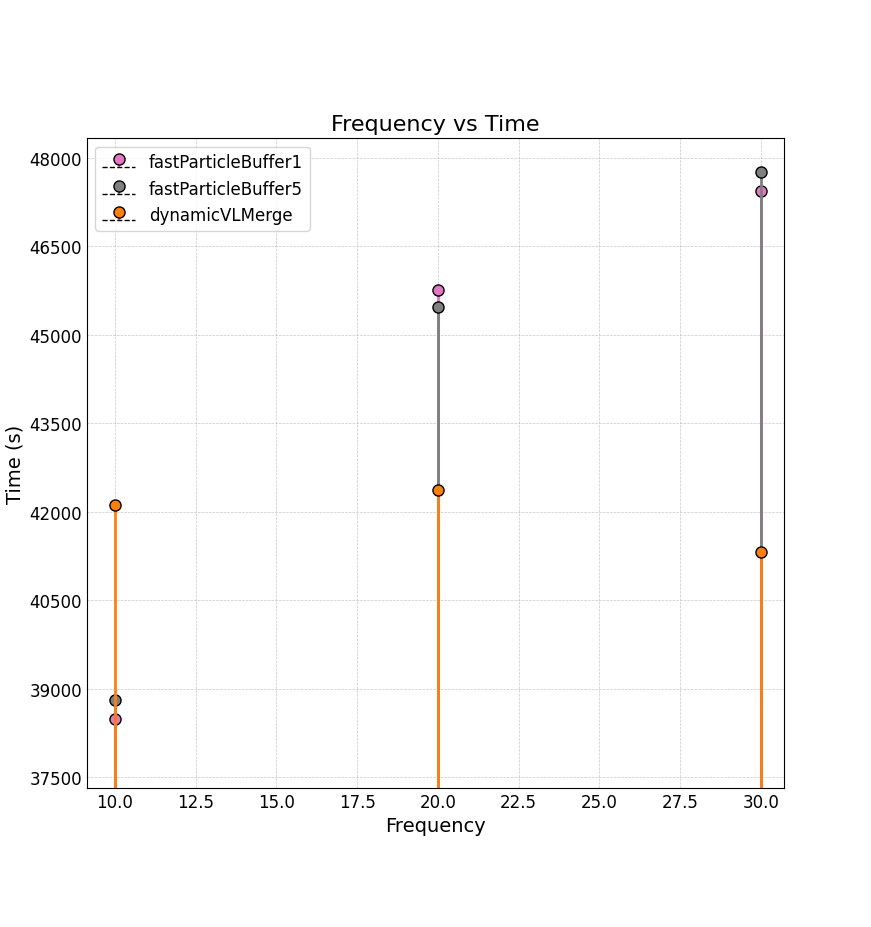
\includegraphics[width=0.8\linewidth]{graphs/spinodalDecomposition/vlcc08_increased.png}
\captionsetup{hypcap=false}
\captionof{figure}{Frequency vs Time for Equilibration with Increased Temperature (vlc\_c08)}
\label{fig:equilibration_plot_increased_temp}
\end{center}


% first of all there are like 300k halo aprticles, so there is already time being spent on remainder traversals bacuse of them, hence the difference in not that much as in the other experiments where there were no halo particles. also for 1 and 5 percent for freq like 30 the 1 percent doesnt even get fullfileed. so why is there a performance difference between 1\% and 5\% threshold??????????

% for the conclusion: if there are halo nice use buffer, if no use it only for non dynamic spots.

% u can either play with the threshold, or choose an appropriate frequency which is big enough, but a threshld is still recommended to cover those times where there is a boom of fast particles in the buffer suddendly. so there should be a sweet spot. at aorund 1\% of particles

% for frequency

\section{Checkpoint Experiments}


Another approach to further investigate the benefits of the particle buffer was to apply it selectively during the least dynamic phase of the simulation. Since remainder traversal is one of the most computationally expensive aspects of the buffer mechanism, the idea was to store particles in the buffer only when the number of fast particles was relatively low.

During the most dynamic phase of the simulation, a large number of fast particles are generated in each iteration, rapidly increasing the number of particles stored in the buffer. Even with a threshold in place, the high number of buffered particles causes remainder traversal times to grow significantly, reducing the overall benefit of avoiding frequent neighbor list rebuilds. However, in the less dynamic phase, where fewer fast particles appear, the remainder traversal overhead should be considerably lower. The hypothesis was that enabling the buffer only during these less dynamic phases could still save neighbor list rebuild time while keeping remainder traversal costs manageable.


To test this hypothesis, the Falling Drop scenario was selected with a 30,000-iteration simulation. Observations showed that after iteration 15,000, the simulation became less dynamic. Based on this, the simulation was divided into two phases:

\begin{itemize}
    \item First 15,000 iterations: The simulation ran without using the buffer.
    \item After iteration 15,000: The buffer was enabled with a 1\% threshold.
\end{itemize}

To enable the transition between the two phases, the last VTK output file from the first phase was used as a checkpoint to initialize the second phase. A VTK output file is a structured XML-based format that stores simulation data, including particle positions, velocities, forces and more.

Figure \ref{fig:checkpoint} illustrates the results of this experiment. To assess the potential improvement, the simulation was Additionally run with a 1\% threshold for the entire 30,000 iterations, allowing for comparison with both the two-phase approach and the Dynamic-VL-Merge branch.  

As shown in the figure, the two-phase approach outperformed the standard 1\% threshold Fast-Particle-Buffer, and ultimately, it also achieved a slightly faster runtime than the Dynamic-VL-Merge branch, although the difference was approximately 1 to 2 seconds. While this improvement may seem small, it suggests that for larger simulations running for several hours, the benefit could become more significant. The effect would likely be more pronounced in longer-running experiments, where reducing remainder traversal costs over extended periods could deliver greater performance gains.

\begin{center}
    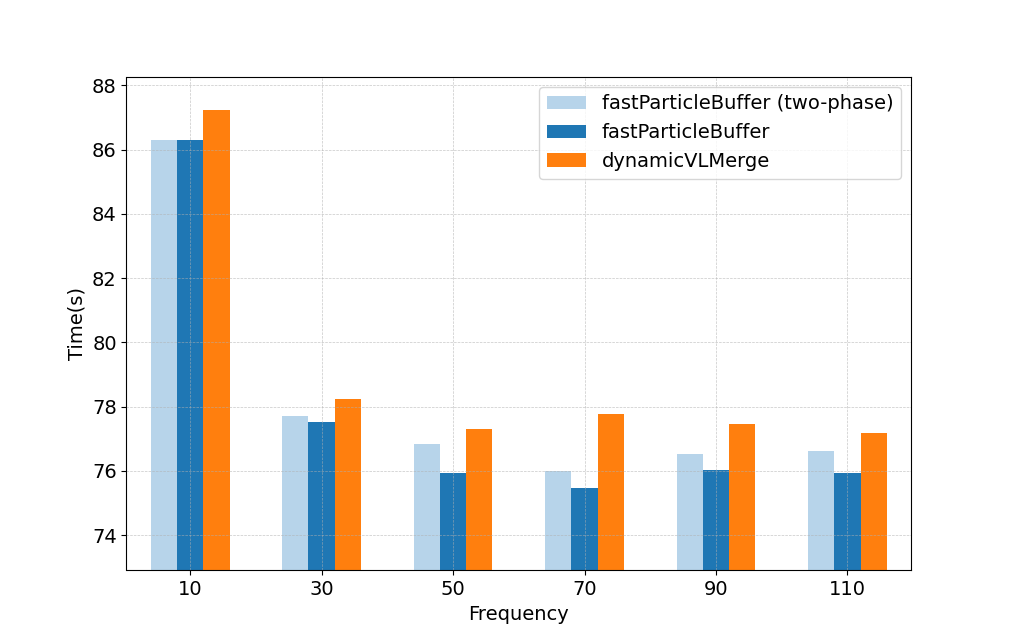
\includegraphics[width=0.8\linewidth]{graphs/checkpoint.png}
    \captionsetup{hypcap=false}
    \captionof{figure}{Chekcpoint Experiments: Frequency vs Time for Falling Drop (vlc\_c08)}
    \label{fig:checkpoint}
\end{center}




